\noindent
Ainsi, l'objectif est de démontrer que le langage assembleur minimal 
présenté est suffisamment puissant pour permettre l'expression d'un 
calcul permettant l'assemblage de blocs deux dimensions à l'aide d'un 
manuel d'instructions.
\medskip

\noindent
Il existe deux formats de manuel d'instructions pouvant être 
interprété par le langage $L'$ :
\begin{enumerate}
  \item \emph{premier format}
    \begin{itemize}
      \item \texttt{1er octet} : largeur (4 bits) et hauteur (4 bits) 
        de la pièce.
      \item \texttt{2e octet} : décalage horizontal (4 bits) et 
        vertical (4 bits) de la pièce.
      \item \texttt{3e octet} : couleur de la pièce.
    \end{itemize}
    Soit par exemple $\texttt{MEM} {:=} [0x11, 0x22, 0x07, 0x21, 0x10, 
    0x06]$ pouvant être traduit par :
    \begin{enumerate}
      \item[1.] Placer une pièce $1 \times 1$ avec un déplacement de 
          $(2, 2)$ et de couleur $0x07$.
      \item [2.] Placer une pièce $2 \times 1$ avec un déplacement de 
          $(1, 0)$ et de couleur $0x06$.
    \end{enumerate}
  \item \emph{deuxième format}
    \begin{itemize}
      \item \texttt{1er octet} : largeur de la pièce.
      \item \texttt{2e octet} : hauteur de la pièce.
      \item \texttt{3e octet} : décalage horizontal de la pièce.
      \item \texttt{4e octet} : décalage vertical de la pièce.
      \item \texttt{5e octet} : couleur de la pièce.
    \end{itemize}
    Soit par exemple $\texttt{MEM} {:=} [0x01, 0x01, 0x02, 0x02, 0x07, 
    0x02, 0x01, 0x01, 0x00, 0x06]$ pouvant être traduit par :
    \begin{enumerate}
      \item[1.] Placer une pièce $1 \times 1$ avec un déplacement de 
          $(2, 2)$ et de couleur $0x07$.
      \item [2.] Placer une pièce $2 \times 1$ avec un déplacement de 
          $(1, 0)$ et de couleur $0x06$.
    \end{enumerate}
\end{enumerate}
Le programme assembleur doit être capable de lire un manuel 
d'instructions (se trouvant dans MEM) dans l'un des deux formats et 
d'assembler les blocs de manière à former une construction en deux 
dimensions.
\medskip

\noindent
Le positionnement suit une logique cumulative : initialement à $(0, 
0)$, soit le coin supérieur gauche, chaque pièce est placée 
relativement à la précédente. Son ancrage est fixé à son coin 
supérieur gauche. Pour que cela reste décidable, la taille de la 
grille servant à y placer les pièces (\texttt{MAP}) est fixée à $8 
\times 8$. Lorsqu'un déplacement occasionne un dépassement de la 
grille, le programme doit repositionner son ancrage à la position
$0$ de cette dimension. C'est-à-dire que si une pièce subit un 
déplacement de $(4, 3)$ et que l'on se trouve à la position $(5, 6)$,
la pièce sera placée à la position $((5 + 4) \mod 8, (6 + 3) \mod 8) 
= (1, 1)$. Cette même logique est appliquée lorsqu'une partie de la 
pièce dépasse la grille. Le point d'ancrage finale après la mise en 
place d'une pièce est donnée par la formule suivante : $((p_{ix}
 + w + dx) \mod 8, (p_{iy} + h + dy - 1) \mod 8)$ où $p_{ix}$ et 
 $p_{iy}$ sont les coordonnées du coin supérieur gauche du point 
d'ancrage initial, $w$ et $h$ sont respectivement la largeur et la
hauteur de la pièce et $dx$ et $dy$ sont les déplacements horizontal
et vertical de la pièce.
\medskip

\noindent
L'illustration ci-dessous montre l'évolution de la grille après le 
placement des pièces pour la mémoire \\
$\texttt{MEM} {:=} [0x11, 0x22, 0x07, 0x21, 0x00, 0x06]$ (premier 
format):
\medskip

\begin{minipage}{0.2\textwidth}
{\scriptsize Initialement : }\\
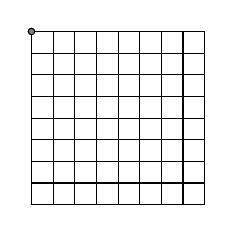
\begin{tikzpicture}[scale=0.275]
  \foreach \x in {0, 1, ..., 7} {
    \foreach \y in {0, 1, ..., 7} {
      \draw[fill=white] (\x, \y) rectangle (\x + 1, \y + 1);
    }
  }

  \draw[fill=gray] (0, 8) circle (0.15);
\end{tikzpicture}
\end{minipage}
\begin{minipage}{0.2\textwidth}
{\scriptsize Après la première pièce :} \\
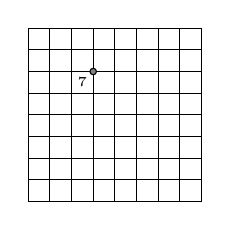
\begin{tikzpicture}[scale=0.275]
  \foreach \x in {0, 1, ..., 7} {
    \foreach \y in {0, 1, ..., 7} {
      \draw[fill=white] (\x, \y) rectangle (\x + 1, \y + 1);
    }
  }

  \draw[fill=gray] (3, 6) circle (0.15);
  \node[font=\tiny] at (2.5, 5.5) {7};
\end{tikzpicture}
\end{minipage}
\begin{minipage}{0.33\textwidth}
  {\scriptsize Après la deuxième pièce :} \\
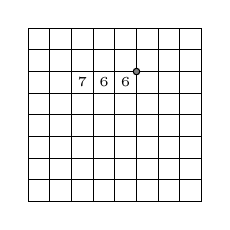
\begin{tikzpicture}[scale=0.275]
  \foreach \x in {0, 1, ..., 7} {
    \foreach \y in {0, 1, ..., 7} {
      \draw[fill=white] (\x, \y) rectangle (\x + 1, \y + 1);
    }
  }

  \draw[fill=gray] (5, 6) circle (0.15);
  \node[font=\tiny] at (2.5, 5.5) {7};
  \node[font=\tiny] at (3.5, 5.5) {6};
  \node[font=\tiny] at (4.5, 5.5) {6};
\end{tikzpicture}
\end{minipage}
\medskip

\noindent
L'objectif est donc dans un premier temps de traduire un manuel 
d'instructions pour en faire une construction dans la grille 
\texttt{MAP}. Dans un second temps, nous conjecturons qu'il existe
plusieurs agencements d'instructions permettant de réaliser un 
programme assembleur minimal $L'$ capable de réaliser cette tâche. Il 
faudrait donc optimiser le programme pour que ce dernier utilise le 
moins de cycle possible avant de terminer la construction.
